\documentclass[german, a4paper, parskip, bibliography=totoc]{scrartcl}

\usepackage[utf8]                   {inputenc}
\usepackage[T1]                     {fontenc}
\usepackage[ngerman]                {babel}
\usepackage[babel, german=quotes]   {csquotes}

\usepackage[backend=bibtex]         {biblatex}
\usepackage                         {color}
\usepackage                         {graphicx}
\usepackage                         {listings}
\usepackage                         {microtype}
\usepackage                         {tikz}
\usepackage                         {tikz-qtree}
\usepackage                         {url}
\usepackage                         {hyperref}

\newcommand{\myAuthor}      {Tim Wiederhake, B.Sc.}
\newcommand{\myTitle}       {JumpVM}
\newcommand{\mySubtitle}    {Java Unified Multi Paradigm Virtual Machine}
\newcommand{\myDate}        {\today}

\author     {\myAuthor}
\title      {\myTitle}
\subtitle   {\mySubtitle}
\date       {\myDate}

\pdfinfo{
    /Author     (\myAuthor)
    /Title      (\myTitle)
    /Keywords   ()
}

\hypersetup{
    pdftitle    =\myTitle,
    pdfauthor   =\myAuthor,
    pdfsubject  ={\myTitle},
    colorlinks  =false,
    pdfborder   =0 0 0
}

\microtypesetup{
    activate    ={true,nocompatibility},
    factor      =1100,
    final,
    kerning     =true,
    shrink      =10,
    spacing     =true,
    stretch     =10,
    tracking    =true
}

\clubpenalty            10000
\widowpenalty           10000
\displaywidowpenalty    10000

\bibliography{report.bib}

\renewcommand{\sfdefault}{ppl}
\renewcommand{\rmdefault}{ppl}
\renewcommand{\ttdefault}{pcr}
\KOMAoptions{DIV=last}

%% Workaround for bug in KOMA-Script 3.12
\usepackage{xpatch}
\makeatletter
\xpatchcmd{\ps@headings}{\sectionmarkformat\fi}{\sectionmarkformat}{}{}
\makeatother
%% /Workaround for bug in KOMA-Script 3.12

\pagestyle{headings}

\lstset{
    language        =Java,
    backgroundcolor =\color{black!8},
    keywordstyle    =\color{red!50!black}\bfseries,
    commentstyle    =\color{blue!60!black},
    numberstyle     =\tiny\color{black!50},
    stringstyle     =\color{},
    showstringspaces=false,
    frame           =none,
    numbers         =left,
    breaklines      =true,
    tabsize         =4,
    emphstyle       =\textbf,
    basicstyle      =\ttfamily,
    numberstyle     =\tiny,
    captionpos      =b
}

\newcommand{\icon}[1]{\includegraphics[scale=.33]{../res/icon32/#1.png}}

\begin{document}
\maketitle

\begin{abstract}
    \noindent JumpVM ist die \enquote{Java Unified Multi Paradigm Virtual
    Machine}: Grafische Oberfläche, Parser, Compiler und Virtuelle Maschine für
    einige verschiedene Programmiersprachen und Programmierparadigmen. Das
    Hauptziel dieser Software ist es, die Vorlesungen \enquote{Einführung in
    den Übersetzerbau} und \enquote{Übersetzung fortgeschrittener
    Sprachkonzepte} an der Universität Ulm zu unterstützen. Die Namen und
    Fähigkeiten der verschiedenen unterstützten Programmiersprachen lehnen sich
    an das Buch \enquote{Übersetzerbau: Theorie, Konstruktion, Generierung}~
    \cite{compilerbau} von R.~Wilhelm und D.~Maurer an, das in den genannten
    Vorlesungen verwendet wird.
\end{abstract}

\vfill{}
\begin{center}
    
\includegraphics[scale=3]{logo.pdf}
\end{center}

\clearpage{}
\tableofcontents{}
\vfill{}
\copyright{} 2015 Tim Wiederhake

Die Weitergabe und Bearbeitung dieses Dokumentes ist unter den Bedingungen der
\enquote{Creative Commons Namensnennung~3.0 Deutschland}-Lizenz gestattet:\\
\href{http://creativecommons.org/licenses/by/3.0/de/}
{http://creativecommons.org/licenses/by/3.0/de/}.
\clearpage{}


%%
%% 1. Einleitung
%%
\section{Einleitung}
Neben den geläufigen imperativen Programmiersprachen gibt es einige weitere
Programmiersprachen, die auf anderen Programmierparadigmen beruhen, etwa
funktionale oder logische Programmiersprachen. Allen gemein ist, dass
Programme, die in diesen Programmiersprachen geschrieben sind, in aller Regel
nicht direkt auf einem Prozessor ausgeführt werden können, sondern erst in
einen zum Prozessor kompatiblen Instruktionssatz übersetzt werden müssen.


\subsection{Motivation}
Der Compilerbau ist diejenige Disziplin der Informatik, die sich mit dem
Entwurf, der Entwicklung und dem mathematischen Unterbau dieser Übersetzer
beschäftigt.

Die hier vorgestellte, im Rahmen einer Projektarbeit an der Universität Ulm
entstandene Software JumpVM soll die Lehre unterstützen und die Übersetzung
unterschiedlicher Programmierparadigmen praktisch erfahrbar machen.


\subsection{Aufbau}
Dieses Dokument ist in sieben Kapitel unterteilt. Nach der Einleitung in
Kapitel~1 wird in Kapitel~2 auf Grundbegriffe und Grundlagen des Compilerbaus
eingegangen. In Kapitel~3 wird eine Bestandsaufnahme der bisherigen
Implementierung der vorlesungsunterstützenden Programme gemacht und die
Probleme mit dieser Implementierung aufgezeigt. Darauf aufbauend werden in
Kapitel~4 Designschwerpunkte und Anforderungen an die zu entwickelnde Software
formuliert. Kapitel~5 widmet sich dem Entwurf und der Entwicklung der Software,
deren Bedienung in Kapitel~6 erläutert wird. Abschließend wird in Kapitel~7
ein Fazit gezogen.


%%
%% 2. Grundlagen
%%
\section{Grundlagen}
In diesem Kapitel werden einige Grundbegriffe und Grundlagen der Arbeitsweise
eines Compilers erläutert.

\paragraph{Lexer, Token}
Aufgabe des Lexers ist es, Quellcode einer bestimmten Programmiersprache
zeichenweise einzulesen und in Symbolen, \enquote{Tokens}, zu gruppieren.
Beispielsweise könnte ein Lexer die Zeichenfolge
\enquote{\texttt{x = 7.4 +y;}} in die folgende Tokenliste übersetzen:

\begin{addmargin}[2em]{2em}
    \ttfamily Bezeichner (x), Zuweisungszeichen, Zahl (7.4),
    Ad\-di\-ti\-ons\-zei\-chen, Bezeichner (y), Befehlstrenner.
\end{addmargin}

\paragraph{Parser, Syntax Tree}
Der Parser verwandelt die lineare Darstellung des Programms als Tokenliste in
einen Syntax Tree, eine Baumstruktur, die der semantischen Struktur des
Programms entspricht. Dieser Baum ist die Grundlage für Optimierungen und
Überprüfungen und könnte für obiges Beispiel folgendermaßen aussehen:

\begin{center}
    \Tree[.Zuweisung [.x ] [.Addition [.7.4 ] [.y ] ] ]
\end{center}

\paragraph{Compiler, Assemblerbefehl}
Der Syntax Tree wird vom Compiler in eine Liste von Assemblerbefehlen
übersetzt. Diese Befehle sind textuelle Darstellungen von Instruktionen eines
bestimmten Prozessors und entsprechen in ihrer Bedeutung dem Quellprogramm.
Eine mögliche Folge von Assemblerbefehlen, die dem oben genannten
Beispielprogramm entsprechen könnten, wäre:

\begin{addmargin}[2em]{2em}
    \ttfamily lda 5, ldc 7.4, lda 6, ind, add, sto.
\end{addmargin}

\paragraph{Assembler, Linker}
Die textuelle Darstellung von Assemblerbefehlen
wird vom Assembler in Maschinencode übersetzt und vom Linker mit eventuellen
anderen Teilen Maschinencode zusammengefügt. Hierbei entsteht ein
lauffähiges, binäres Programm.

\paragraph{Virtual Machine}
Existiert der Prozessor zum Ausführen eines
Programms nicht real, sondern selber nur als Software, so spricht man von
einer Virtuellen Maschine. Da reale Prozessoren zunehmend komplexer werden,
eignen sich Virtuelle Maschinen besonders, um in der Lehre die Funktionsweise
eines Compilers bzw. Assemblers zu verdeutlichen. Die Instruktionen einer
Virtuellen Maschine sind selber definierbar und an die gewählte Quellsprache
anpassbar.


%%
%% 3. Bestandsaufnahme
%%
\section{Bestandsaufnahme}
In den Linux-Rechnerpools der SGI sind für die Abteilung Compilerbau im
Verzeichnis \texttt{/opt/Abteilungen/pm/} mehrere Programme installiert.
Diese sind mit Tk-Gofer~2.0 programmiert und stammen aus den Jahren 1995--1996
(mama) und 1998 (pmach); für wim konnte keine Datierung gefunden werden.

Gofer ist ein Haskell-Dialekt, der seit 1999 nicht weiterentwickelt
wird~\cite{url_gofer} und auf den Rechnern, auf denen
das Betriebssystem Ubuntu Linux 13.10, Kernel 3.11.0-18 läuft, nicht aus den
Repositories installierbar. Daher liegt im angegebenen Verzeichnis eine
selbsterstellte Gofer/Tk-Gofer-Installation.

Tk ist ein Toolkit zur Entwicklung von grafischen Benutzeroberflächen,
entwickelt für die Scriptsprache Tcl. Die Tk-Gofer Installation empfiehlt die
Version 4.2 oder höher für Tk und Version 7.6 oder höher für Tcl. Die
niedrigste Version der Softwarepakete Tcl und Tk in den Ubuntu-Repositories
ist Version 8.5.

Die Programmiersprache Haskell liegt im Tiobe-Index der populärsten
Programmiersprachen (Stand: Oktober 2014) auf Platz 40 mit einem Rating von
0,341\%~\cite{url_tiobe}. Die Programmiersprache Gofer ist im Ranking nicht
vertreten. Davon ausgehend kann angenommen werden, dass die Zahl der
Programmierer, die Goferprogramme warten können, äußerst gering ist. Die
Verwendung einer selbstgeschriebenen Bibliothek zur Anbindung von Gofer an
Tk/Tcl erschwert die Wartbarkeit der vorliegenden Programme weiter.

Installieren lassen sich diese Programme etwa unter Windows oder MacOS
gar nicht, unter Linux nur mit einigem Aufwand. Beispielsweise sind die in
Debian 8 (Jessie) vorzufindenden Bibliotheken libtk8.5 und libtcl8.5 mit den
Programmen inkompatibel.

Des Weiteren ist die Lizenzierung der urspünglichen Programme unbekannt, daher
muss vom restriktivsten Fall ausgegangen werden, der keine Installation auf
einem eigenen Rechner erlaubt. Dies ist ungünstig, wenn die Programme für den
Übungsbetrieb einer Vorlesung eingesetzt werden sollen und nur an einer sehr
eingeschränkten Zahl Computern benutzbar sind.


\subsection{pmach}
\begin{figure}[htb]
    \centering
    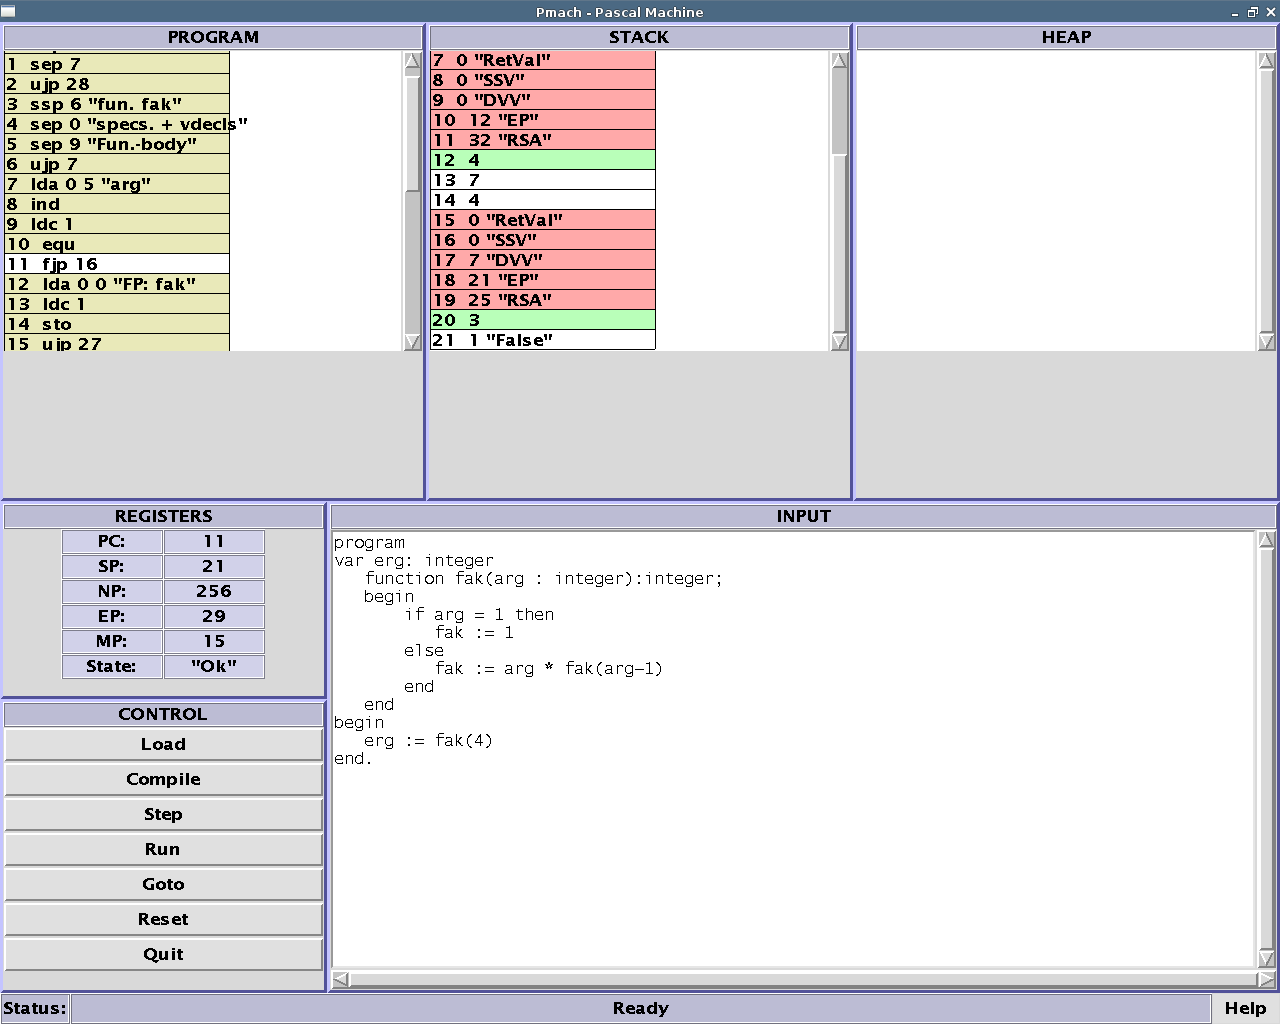
\includegraphics[width=\textwidth]{screenshot_old_pmach.png}
    \caption{Die pmach beim Ausführen eines Beispielprogramms.}
    \label{img_gofer_pmach}
\end{figure}

Abbildung~\ref{img_gofer_pmach} zeigt das Programm pmach. In der oberen Hälfte
des Fensters werden die Programminstruktionen des compilierten
Beispielprogramms, der Stack und der Heap des aktuell laufenden Programms
angezeigt. Die Programminstruktionen sind teilweise mit Abkürzungen annotiert.
Die Instruktion \texttt{lda 0 0 "FP: fak"} bezieht sich etwa auf die
Framepointer der Funktion \enquote{fak}. Ähnlich sind die organisatorischen
Zellen der einzelnen Frames auf dem Stack beschriftet, zusätzlich werden diese
und die Zellen, die lokale Variablen enthalten, jeweils farblich hervorgehoben.

Die untere Hälfte des Fensters beinhaltet eine Übersicht über die Register
der Virtuellen Maschine und ihren jeweiligen Wert. Darunter befinden sich
einige Schaltflächen, die der Steuerung des Programms dienen, etwa dem Laden,
Speichern, Compilieren und Ausführen von Programmen. Rechts davon ist ein
Eingabefeld zu sehen, in dem der Quellcode des aktuellen Programms angezeigt
wird und geändert werden kann.

Eine Statuszeile zeigt den momentanen Zustand der VM an (etwa \enquote{Ready}
oder \enquote{Running program ...}), ein Klick auf die Schaltfläche
\enquote{Help} zeigt ein Fenster mit der verwendeten Grammatik für die
Übersetzung der Programme in EBNF-Syntax an und beschreibt kurz die verfügbaren
Schaltflächen und verwendeten Farben.

Ein Fehler in der pmach sorgt dafür, dass boolesche Werte falsch angezeigt
werden. Die Größe der einzelnen Bereiche \enquote{Program}, \enquote{Stack}
etc. passen sich teilweise nicht der tatsächlichen Fenstergröße an, wodurch
immer maximal 15 Einträge des jeweiligen Speichers sichtbar sind. Die
Ausführung größerer Programme verlangsamt sich mit jedem Schritt; ab einer
bestimmten Länge der Ausführung oder beim Übersetzen größerer Programme beendet
sich das Programm aufgrund von Speichermangel mit folgender Fehlermeldung im
Terminal:

\begin{addmargin}[2em]{2em}
    \ttfamily ERROR: Garbage collection fails to reclaim sufficient space
\end{addmargin}


\subsection{mama}
\begin{figure}[htb]
    \centering
    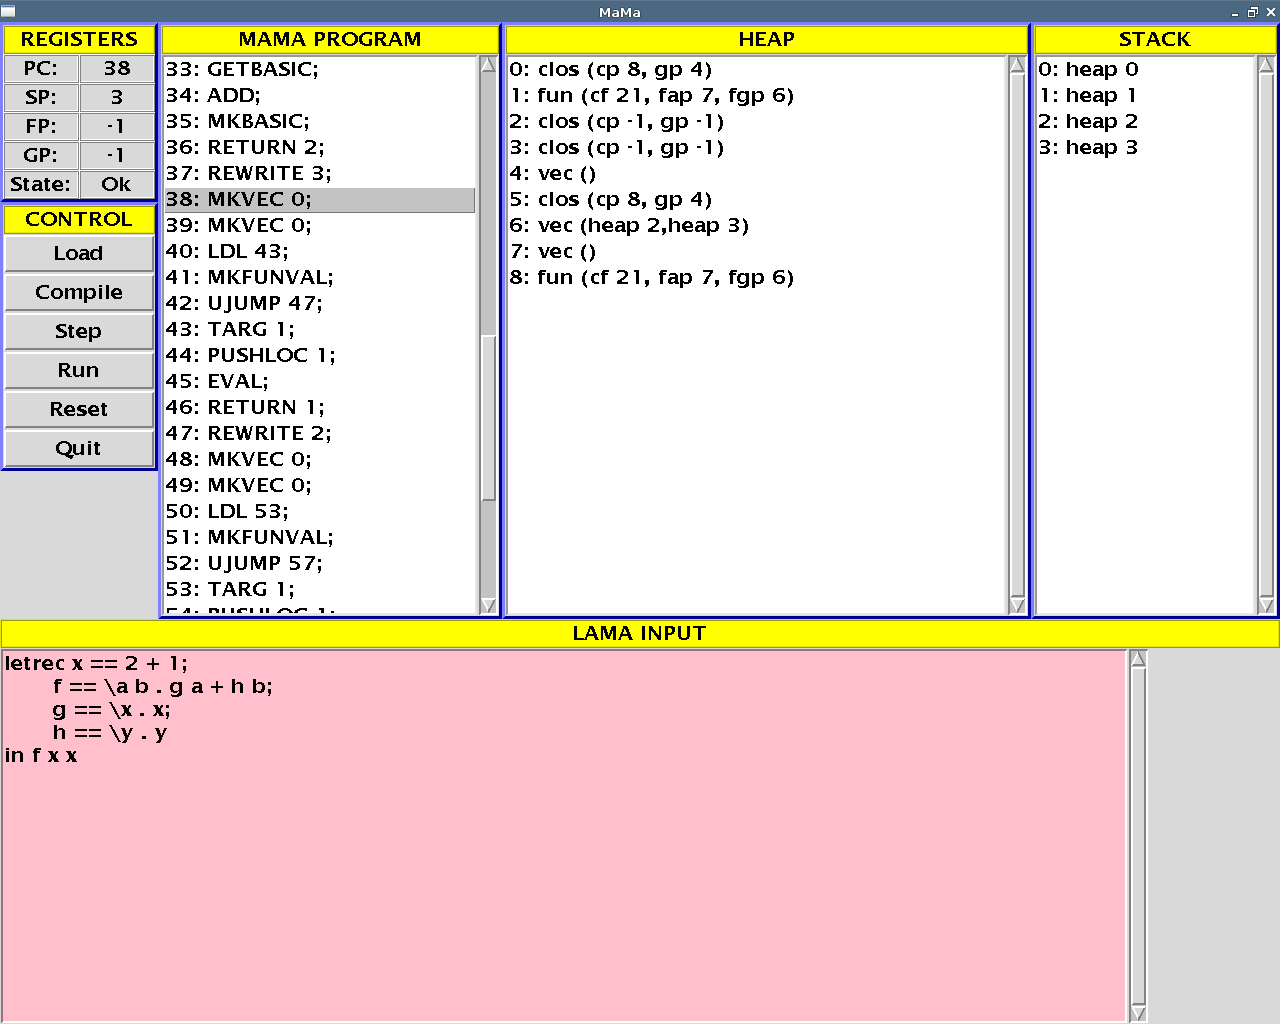
\includegraphics[width=\textwidth]{screenshot_old_mama.png}
    \caption{Die mama beim Ausführen eines Beispielprogramms.}
    \label{img_gofer_mama}
\end{figure}

Abbildung~\ref{img_gofer_mama} zeigt das Programm mama. In der oberen Hälfte
des Programms wird, wie bei der pmach, der Inhalt des Speichers angezeigt,
allerdings mit vertauschter Reihenfolge von Stack und Heap.

Die Registeranzeige und die Kontrollschaltflächen finden sich hier in
der oberen Hälfte des Fensters, im Gegensatz zur pmach. Die Schaltfläche
\enquote{Goto} fehlt. Die Elemente im Speicher werden nicht eingefärbt und bei
der Benutzung des Programms fällt auf, das der Versuch syntaktisch inkorrekte
Programme zu übersetzen zum Beenden des Programms führt. Eine Fehlermeldung
wird nur im Terminal ausgegeben, beispielsweise:

\begin{addmargin}[2em]{2em}
    \ttfamily Program error: unknown identifier z
\end{addmargin}


\subsection{wim}
\begin{figure}[htb]
    \centering
    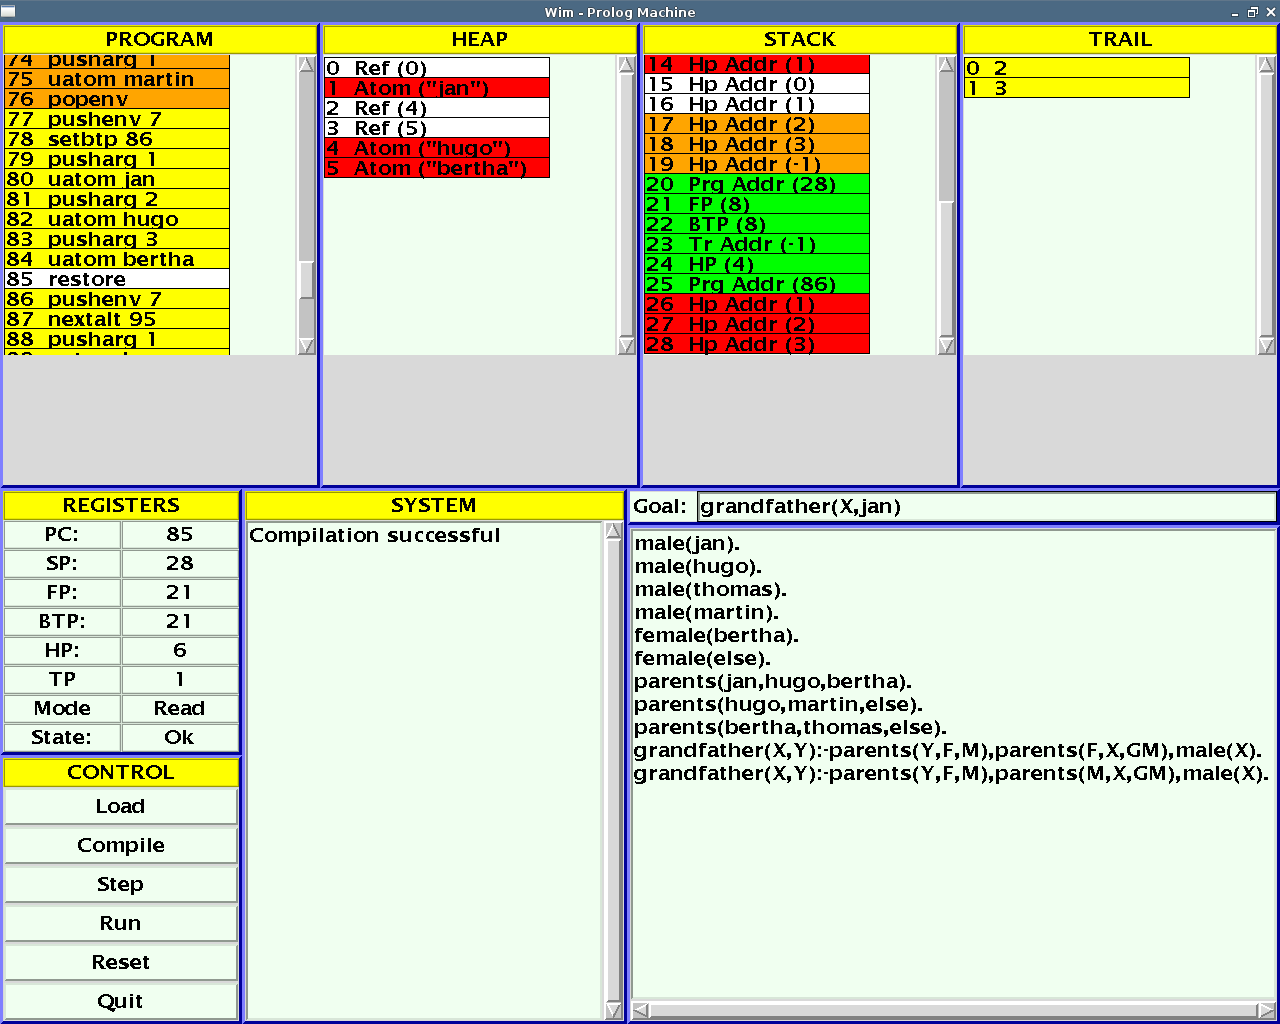
\includegraphics[width=\textwidth]{screenshot_old_wim.png}
    \caption{Die wim beim Ausführen eines Beispielprogramms.}
    \label{img_gofer_wim}
\end{figure}

Abbildung~\ref{img_gofer_wim} zeigt das dritte Programm wim. Wieder finden sich
in der oberen Hälfte des Fensters die Inhalte der verschiedenen
Speicherbereiche, ohne Kommentare, dafür eingefärbt. Die Farbgebung wird nicht
erläutert. In der unteren Hälfte des Fensters befinden sich die
Schaltflächen zur Steuerung des Programms, die Registerübersicht und ein
Textfeld zur Eingabe des Programms. Zusätzlich ist ein Feld vorhanden, in dem
Ausgaben angezeigt werden, etwa Meldungen zur erfolgreichen Übersetzung eines
Programms oder Ausgaben durch die Ausführung des Programms.

Das Eingabefeld für Programmtext ist zweigeteilt. Das Ziel (\enquote{Goal})
eines wim-Programms kann nicht zusammen mit seinem restlichen Quelltext
gespeichert oder geladen werden. Leerzeichen im Quelltext werden als
syntaktische Fehler betrachtet.

Außerdem scheint die Ausführung von wim-Programmen fehlerhaft zu sein,
beispielsweise erzeugt die Ausführung des Programms mit der Faktenbasis
\enquote{equal(X,X).} und dem Ziel \enquote{equal(a,b)} die Ausgabe
\enquote{Yes}.


%%
%% 4. Designziele
%%
\section{Designziele}
Für die Entwicklung eines Nachfolgers ergeben sich aus der Untersuchung der
Programme, ihrer Stärken und Schwächen, einige Schwerpunkte und Designziele:

\paragraph{Plattformunabhängigkeit und Portabilität}
Als Werkzeug der Übung und zur Unterstützung der Vorlesung soll das Programm
auf allen verwendeten Plattformen des Dozenten, der Hilfskräfte und der
Studenten lauffähig sein. Das Programm soll ohne Installation lauffähig sein.

\paragraph{Freizügige Lizenzierung}
Die Lizenzierung der Software muss es den Studenten erlauben, die Software auf
einem eigenen Rechner mindestens für die Dauer des Besuches der Vorlesung zu
verwenden.

\paragraph{Benutzerfreundlichkeit}
Die Dokumentation der Software muss es den Benutzern erlauben, die Handhabung
und die Funktionsweise des Programms zu verstehen. Verwendete Symbolik, wie
etwa farbliche Hervorhebungen, muss selbsterklärend sein oder explizit
erläutert werden. Fehleingaben müssen abgefangen werden, Fehlermeldungen auf
die Art des Fehlers oder die erwartete Eingabe hinweisen.

\paragraph{Wartbarkeit}
Die Software soll in einer Programmiersprache geschrieben sein, die aufgrund
hoher Verbreitung oder einfacher Erlernbarkeit Änderungen und Korrekturen durch
Dritte in der Zukunft erlauben. Die Anwendung von Best Practices aus dem
Bereich des Software Engineering soll die Qualität der Software maximieren.


%%
%% 5. Entwicklung
%%
\section{Entwicklung}
Ausgehend von den in Kapitel 4 genannten Anforderungen wurde im Wintersemester
2013 und Sommersemester 2014 die Software JumpVM entwickelt.

Als Programmiersprache wurde Java gewählt, da Java-Programme auf allen zu
erwartenden Plattformen (Windows, MacOS, Linux) lauffähig sind und ohne
zusätzliche Softwarebibliotheken grafische Oberflächen auf allen diesen
Plattformen erzeugen können. Java ist im Vergleich zu etwa in C oder C++
weniger performant. Da die Anforderungen an die Benutzerhardware als gering
eingeschätzt wurden, ist dies vernachlässigbar.

Eine Recherche zu verwendbaren, bereits existierenden Bibliotheken zum Parsen,
Compilieren und Ausführen von Programmen und der Entwicklung von
Programmiersprachen brachte zwei interessante Ergebnisse:

LLVM (\enquote{Low Level Virtual Machine}) ist eine Sammlung von modularen und
wiederverwendbaren Compiler- und Toolchain-Technologien~\cite{url_llvm}.
Herzstück ist die LLVM-IR (\enquote{LLVM Intermediate Representation}), eine
architekturunabhängige Pseudo-Assem\-blersprache. LLVM enthält eine Vielzahl an
Modulen, die Code in LLVM-IR optimieren und in Assemblerprogramme für
unterschiedlichste Plattformen übersetzen kann. Die Verwendung von LLVM wurde
allerdings auf Grund des unüberschaubaren Aufwandes, mehrere Backends für
LLVM zu entwickeln, verworfen.

ANTLR (\enquote{ANother Tool for Language Recognition}) ist, wie etwa auch
YACC (\enquote{Yet Another Compiler Compiler}), ein
Parsergenerator~\cite{url_antlr}: Aus einer formal definierten Grammatik werden
Lexer und Parser für diese Grammatik erzeugt. Zusätzlich stehen einige
Werkzeuge und eine grafische Oberfläche namens ANTLRWorks für die
Erstellung der Grammatik zur Verfügung.

Da für die zu erstellenden Parser keine Grammatiken zur Verfügung standen
bzw.\ die Grammatik der pmach inkonsistent war, wurden die Grammatiken mit
ANTLRWorks erstellt. Insbesondere die Möglichkeit des automatischen Testens
der Grammatiken und die grafische Darstellung der einzelnen Produktionen einer
Grammatik erwiesen sich als äußerst nützlich. Abbildung~\ref{img_antlr} zeigt
einige Beispiele für die grafische Darstellung von Produktionen aus den
entstandenen Grammatiken.

\begin{figure}[htb]
    \centering
    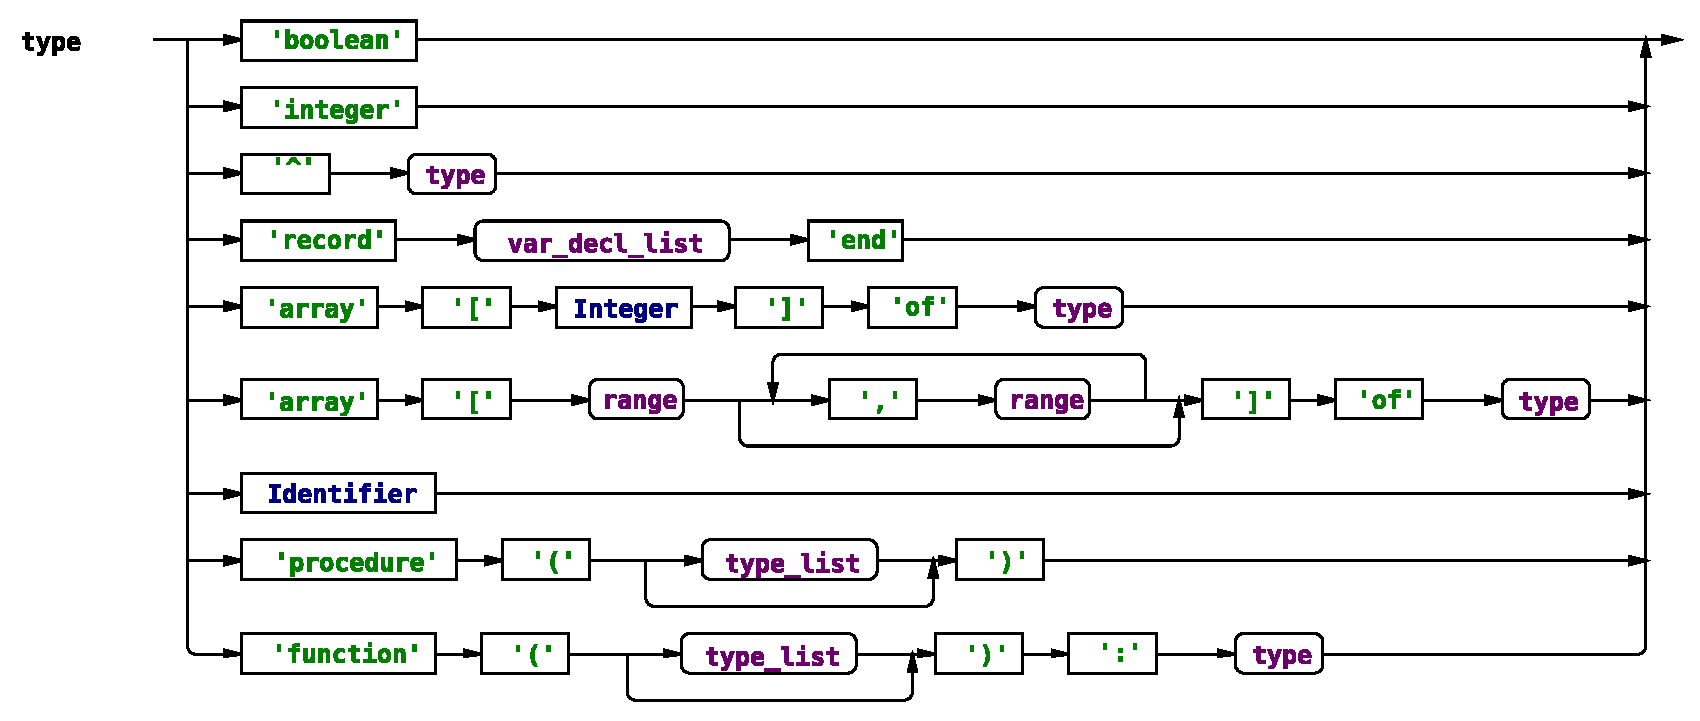
\includegraphics[width=\textwidth]{antlrworks_pama_type.pdf}
    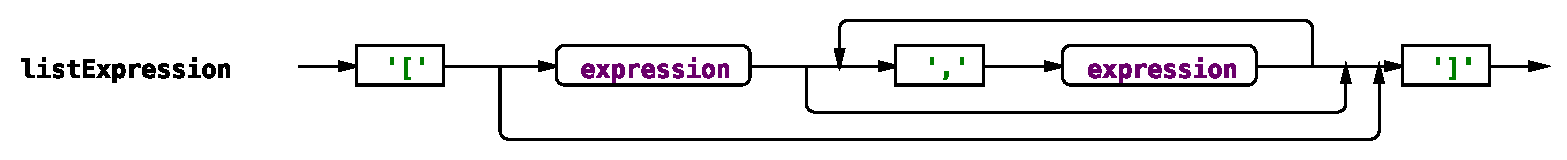
\includegraphics[width=\textwidth]{antlrworks_mama_listexpression.pdf}
    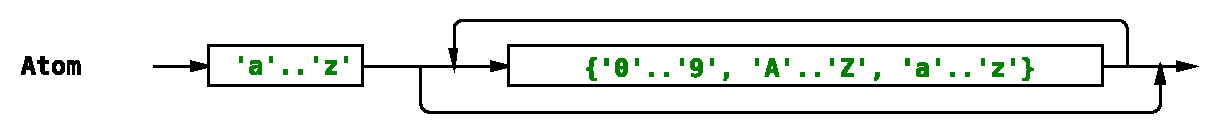
\includegraphics[width=\textwidth]{antlrworks_wima_atom.pdf}
    \caption{Grafische Darstellung einiger Produktionen in ANTLRWorks. Die
        zugehörigen Grammatiken liegen der Software bei.}
    \label{img_antlr}
\end{figure}

Letztendlich wurde der Einsatz des ANTLR Parsergenerators in der zu
erstellenden Software verworfen, da die generierten Lexer und Parser zu komplex
waren und sich nicht an die gewünschte Funktionalität anpassen ließen. Auf
Basis der mit ANTLRWorks erstellten Grammatiken wurden daher händisch einfache
Recursive Descent Parser entwickelt.

Die Beispielprogramme der bestehenden Implementation wurden entnommen,
ergänzt und als Testfälle für Unit-Tests der einzelnen Komponenten (Lexer,
Parser, Compiler und VM) verwendet. So konnte sichergestellt werden, dass die
Software die gleichen Daten wie die bisherigen Implementationen produziert,
also die gleichen Maschinenbefehle aus dem gleichen Quelltext erzeugt.
Abbildung~\ref{img_jumpvm_junit} zeigt das Ergebnis eines solchen Testlaufs:
Für jede Beispieldatei stimmen die Ergebnisse von Lexer, Parser, Compiler und
Ausführung des Programms mit den erwarteten Ergebnissen überein.

\begin{figure}[htb]
    \centering
    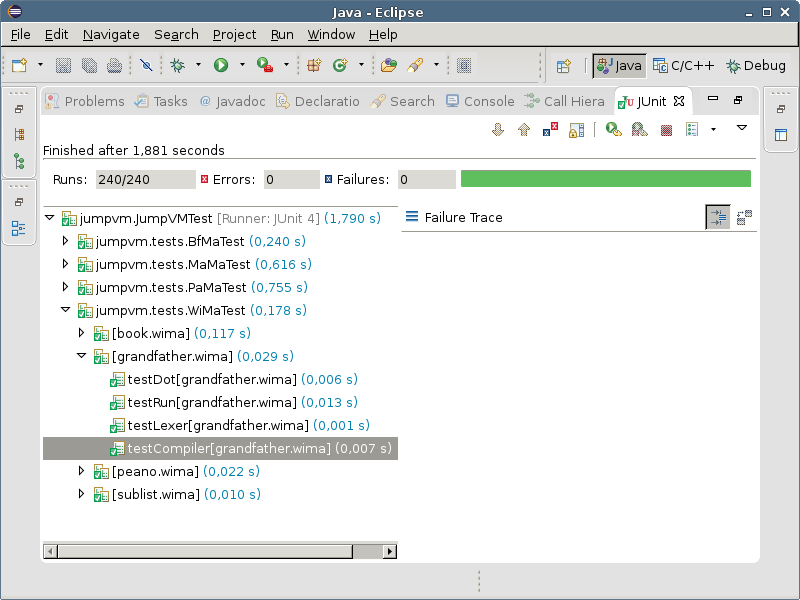
\includegraphics[width=\textwidth]{screenshot_junit.png}
    \caption{Testen der Software mit JUnit.}
    \label{img_jumpvm_junit}
\end{figure}

Checkstyle~\cite{url_checkstyle} ist ein Werkzeug für statische Codeanalyse von
Java-Programmen, mit dem die Einhaltung von Programmierstandards überprüft
werden kann. Häufige Fehler können so erkannt und behoben werden. Die Spanne
der erkannten Fehler reicht vom direkten Vergleich von Zeichenketten mit dem
\enquote{==}-Operator (statt \enquote{equals}) bis zu Verletzungen der
Prinzipien objektorienterten Designs (wie etwa mangelnde Datenkapselung) und
fehlender Dokumentation. Um die Qualität des Quellcodes zu erhöhen, wurden alle
von Checkstyle erkannten Mängel behoben.

Die Dokumentation des Quellcodes erfolgt mit dem Java-eigenen Werkzeug
JavaDoc. In Kombination mit Checkstyle kann so sichergestellt werden, dass jede
Klasse, Funktion und Klassenfeld für Änderungen und Korrekturen durch Dritte
dokumentiert und in ihrer Funktion beschrieben ist. Abbildung
\ref{code_javadoc} zeigt exemplarisch die Kommentierung einer Funktion der
Klasse \enquote{jumpvm.compiler.Parser}. Durch den formellen Aufbau der
Kommentare ist es möglich, die gesamte Code-Dokumentation beispielsweise im
HTML oder PDF-Format zu extrahieren und konvertierten.

\begin{figure}[htb]
    \begin{lstlisting}[gobble=4]
    /**
    * Discard {@code expectedToken} and read next token.
    *
    * @param expectedToken expected token
    * @throws ParseException if current token != expected token
    */
    protected final void eat(final T expectedToken) throws ParseException {
        expect(expectedToken);
        token = lexer.nextToken();
    }
    \end{lstlisting}
    \caption{Kommentierung mit JavaDoc.}
    \label{code_javadoc}
\end{figure}

Zur möglichst einfachen Verwendung wurde die gesamte Software unter die
\enquote{GNU General Public License} in der Version 3 oder höher gestellt.
Diese Lizenzierung ermöglicht es jedem Anwender, die Software nach Belieben zu
nutzen, kopieren oder weiterzuentwickeln. Dies kommt besonders Nutzern im
akademischen Bereich zu Gute, da es das Untersuchen der Software, um sie
verstehen zu lernen, explizit erlaubt und die Weiterentwicklung vereinfacht.

Die Software ist modular angelegt, mit generischen Lexer-, Parser- und
Compiler-Funk\-ti\-on\-en, die von den Modulen der einzelnen Übersetzern und
Virtuellen Maschinen verwendet und angepasst werden können. Die Organisation
des JumpVM-Quellcodes ist in Kapitel 5.5 genauer erläutert. Die Verwendung der
generischen Klassen erlaubt es, die Oberfläche des Programms einheitlich zu
gestalten.

Durch diese Modularisierung und Vereinheitlichung der Schnittstellen war es
möglich, einige neue Funktionen, die in der bisherigen Implementierung nicht
existierten, in die Software einzubauen. Unabhängig vom verwendeten Modul kann
die Ausführung eines Programms schrittweise rückgängig gemacht werden, um den
Effekt einer Instruktion genauer zu untersuchen. Die Werte der Register und
Speicherzellen lassen sich auch während der Ausführung ändern, um das Austesten
von \enquote{Was wäre wenn\ldots{}}-Szenarien zu erlauben. Das Konzept der
teilweise annotierten Speicherzellen der pmach wurde übernommen und erweitert:
Jede Speicherzelle ist zum besseren Verständnis mit ihrer jeweiligen Bedeutung
und ihrem Datentyp annotiert. Beispielsweise könnte eine Speicherzelle
anzeigen, dass es sich bei ihrem Wert um einen Zeiger in den Programmspeicher
(Datentyp) auf die Funktion \enquote{f} (Bedeutung des Wertes) handelt.

Eine weitere Verbesserung gegenüber der vorherigen Implementierung ist die
interaktive Zuordnung von Quellcode eines Programms, seinem Syntaxbaum und den
produzierten Instruktionen des Maschinencodes. Sie erlaubt es dem Benutzer
unmittelbar nachzuvollziehen, welcher Teil seines Quellcodes zu welchen
Instruktionen geführt hat. Abbildung~\ref{img_jumpvm_run} zeigt, wie diese
Zuordnung im fertigen Programm umgesetzt wird: Zusammengehörende Instruktionen,
Knoten im Syntax-Baum und Abschnitte im Quellprogramm sind jeweils identisch
eingefärbt.

Die Syntax der Programmiersprachen der bisherigen Implementierung wurde um
Befehle zur Ein- und Ausgabe von Daten erweitert, um die möglichen Programme
für die Benutzer interessanter machen zu können.

\begin{figure}[htb]
    \centering
    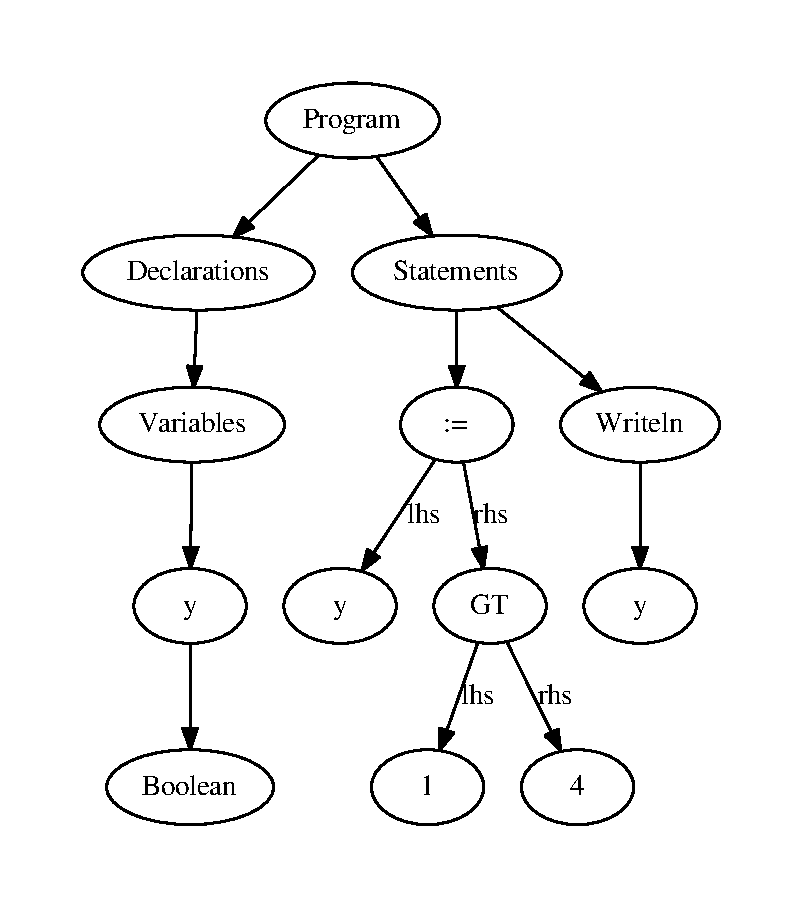
\includegraphics[width=0.5\textwidth]{p13_pama_dot.pdf}
    \caption{Darstellung eines Programms als Syntaxbaum.}
    \label{img_dot}
\end{figure}

Um die Software auch als Werkzeug zur Vorlesungsvorbereitung attraktiv zu
machen und den Datenaustausch mit anderen Programmen zu ermöglichen, wurden
Funktionen zum Export des Syntax-Baumes als
Graphviz-DOT-Dateien~\cite{url_graphviz} implementiert, wie etwa in
Abbildung~\ref{img_dot} zu sehen. Zusätzlich ist der Export des momentanen
Zustandes der laufenden Virtuellen Maschine im XML-Format möglich.

\subsection{PaMa}
Das Modul PaMa ist in der Lage, Programme in einer Pascal-ähnlichen,
imperativen Sprache zu übersetzen und auszuführen. Abbildung~\ref{code_pama}
zeigt das Beispielprogramm \enquote{fak.pama}, das die Fakultätsfunktion
berechnet.

\begin{figure}[htb]
    \lstinputlisting[language={Pascal}] {../res/source/fak.pama}
    \caption{Rekursive Berechnung der Fakultätsfunktion.}
    \label{code_pama}
\end{figure}

PaMa wurde gegenüber pmach um Funktionen zur Ein- und Ausgabe von
Daten (\texttt{readln} und \texttt{writeln}) erweitert. Die fehlerhafte
Darstellung von Booleschen Werten wurde korrigiert und die Setzung von
\enquote{;} (Semikolon) im Deklarationsteil von Funktionen und Prozeduren
vereinheitlicht.

Während Pascal noch einige weitere Datentypen kennt, sind die einzigen
primitiven Datentypen dieser Programmiersprache die Ganzzahl (\texttt{integer})
und der Wahrheitswert (\texttt{boolean}). Darüber hinaus sind zusammengesetzte
Datentypen (\texttt{record}), Felder (\texttt{array}) und Zeiger
(\texttt{pointer}) möglich.

Vor der Übersetzung der Programme werden diese auf Typkorrektheit geprüft. So
werden Fehler gefunden, die die syntaktische Analyse durch den Parser nicht
aufspüren kann, etwa die Zuweisung eines ganzzahligen Wertes an eine Variable
vom Type Wahrheitswert.

Der Compiler eröffnet für jede Prozedur / Funktion des Programms
einschließlich der Hauptprozedur eine Übersetzungsumgebung, die Informationen,
etwa zur Positionierung von Variablen im Speicher beinhaltet. Nun werden die
einzelnen Anweisungen der Prozeduren übersetzt.

Während des Übersetzens wird zwischen dem sogenannten Linkswert und dem
Rechtswert einer Variable bzw.\ eines formellen Ausdrucks unterschieden. Der
Rechtswert bezeichnet den tatsächlichen Wert eines Ausdrucks und könnte etwa
\enquote{5} für den Ausdruck \enquote{x} sein, oder \enquote{7} für den
Ausdruck \enquote{3 + 4}. Der Linkswert bezeichnet eine Adresse im Speicher und
wird benötigt, um dem bezeichneten Datum einen neuen Wert zuzuweisen. Für den
Ausdruck \enquote{x} könnte der Linkswert, also die Adresse der Variable,
\enquote{17} sein. Für den Ausdruck \enquote{3 + 4} exisitiert kein Linkswert:
Diesem Ausdruck kann kein neuer Wert zugewiesen werden und er hat keinen
benannten Platz im Speicher.

Die Virtuelle Maschine, die die übersetzten PaMa-Programme ausführt, ist eine
Stackmaschine. Werte werden auf dem Stack manipuliert, statt wie etwa bei
x86-Prozessoren in Registern gehalten. Dies ermöglicht eine sehr einfache
Übersetzung und Virtuelle Maschine geringer Komplexität. Da bei
Stackmaschinen sehr viele Speicheroperationen durch die Manipulation des Stacks
anfallen, sind diese allerdings weniger Effizient als Registermaschinen, die
einige Werte in Registern zwischenspeichern können.


\subsection{MaMa}
Das Modul MaMa übersetzt und führt Programme in einer funktionalen,
Haskell-ähnlichen Sprache aus. Abbildung~\ref{code_mama} zeigt das
Beispielprogramm \enquote{example01.mama}, in dem eine Lambda-Funktion
definiert und aufgerufen wird.

\begin{figure}[htb]
    \lstinputlisting[language={Haskell}, morekeywords={letrec}]
        {../res/source/example01.mama}
    \caption{Definition einer Lambda-Funktion.}
    \label{code_mama}
\end{figure}

MaMa-Programme stellen jeweils einen zu berechnenden Ausdruck dar. Im obigen
Beispiel etwa soll der Audruck \enquote{f 3 a} berechnet werden, wobei
Definitionen für \enquote{f} und \enquote{a} gemacht werden, die wiederum
rekursiv Ausdrücke enthalten können.

Die MaMa-VM ist wie die PaMa-VM eine Stackmaschine. Allerdings werden hier
nicht die Werte direkt, sondern Zeiger auf Speicherzellen im Heap auf den Stack
gelegt. Dieser Zeiger kann nun auf einen Wert oder eine Funktion, die den Wert
des Ausdrucks berechnet (\enquote{Closure}), zeigen. Nach dem Auswerten der
Closure wird der berechnete Wert an der passenden Speicherzelle für
zukünftige Zugriffe gespeichert, damit der Ausdruck nicht mehrfach berechnet
werden muss.


\subsection{WiMa}
Das Modul WiMa kann Programme in einer logischen, Prolog-ähnlichen Sprache
übersetzen und ausführen. Abbildung~\ref{code_wima} zeigt das Beispielprogramm
\enquote{peano.wima}, in dem die Peano-Arithmetik mit logischen Klauseln
nachgebildet wird und die Anfrage \enquote{Welche Zahl erfüllt die Anforderung,
dass sie die zweite Potenz der Zahl Drei ist?} beantwortet.

\begin{figure}[htb]
    \lstinputlisting[language={Prolog}, otherkeywords={?-,:-,.}]
        {../res/source/peano.wima}
    \caption{Peano-Arithmetik.}
    \label{code_wima}
\end{figure}

Das Ausführen eines solches Programms bewirkt nun, dass geprüft wird, ob die
Anfrage aus der bestehenden Datenbasis, genannt Fakten, geschlussfolgert werden
kann, also die Anfrage gemäß der Datenbasis wahr ist und für welche
Variablenbelegungen dies der Fall ist.

Dafür wird bei der Übersetzung Code generiert, der versucht, die gegebenen
Fakten mit der jeweiligen Teilanfrage in Übereinstimmung zu bringen
(\enquote{unifizieren}). Die dafür getroffenen Annahmen über die
Variablenbelegung werden in einem separaten Speicher vorgehalten, um sie, im
Falle eines Widerspruchs, also der Unmöglichkeit Anfrage und Fakten zu
unifizieren, einfach rückgängig machen zu können.

Der Befehlssatz der WiMa ist von den bisher vorgestellten Befehlssätzen der
wahrscheinlich hardware-fernste. Er enthält die komplexesten Instruktionen die
deutlich sichtbar an die Quellsprache angepasst sind. Ebenfalls fällt auf,
dass die WiMa-VM über ein ungewöhnliches Register (\enquote{Modus}) verfügt,
das keine numerischen Werte annimmt sondern nur die Zustände \enquote{read}
und \enquote{write} kennt.


\subsection{BfMa}
Um die Modularisierung der Software zu testen und die Anwendungsmöglichkeiten
der Software zu demonstrieren, wurde ein weiteres Modul für eine
ungewöhnliche Programmiersprache entwickelt.

\enquote{Brainfuck} ist eine sogenannte \enquote{esoterische}
Programmiersprache, die nicht ernsthaft für die Entwicklung größerer
Programme gedacht ist. Das Ziel dieser Sprache ist es, durch möglichst kleinen
Befehlsumfang den kleinstmöglichen Übersetzer zu ermöglichen. Das Programmieren
in Brainfuck ähnelt dem direkten Programmieren einer Turing-Maschine und
ist sehr unübersichtlich, was zum Namen der Sprache führte.

Da diese Sprache über nur acht Befehle verfügt eignet sie sich optimal, um die
Verwendung der generischen JumpVM-Funktionen zum Parser- bzw.\ Compilerbau zu
demonstrieren, ohne durch ihre Komplexität abzulenken.


\subsection{Organisation des JumpVM Quellcodes}

Der JumpVM-Quellcode~\cite{url_jumpvm} ist in sieben Verzeichnisse, in Java
\enquote{Packages} genannt, aufgeteilt. Diese Packages enthalten:

\begin{itemize}
\item \emph{ast:}
    Datenstrukturen, aus denen die Syntaxbäume der zu übersetzenden Programme
    zusammengesetzt werden.
\item \emph{code:}
    Die Implementation der Maschinenbefehle der Virtuellen Maschinen.
\item \emph{compiler:}
    Lexer, Parser und Hilfsklassen, die Quelltext in Syntaxbäume und
    Maschinenbefehle umwandeln.
\item \emph{exception:}
    Hilfsklassen für die Fehlerbehandlung und Präsentierung.
\item \emph{gui:}
    Die Grafische Oberfläche des Programms.
\item \emph{memory:}
    Klassen für Speicher und Speicherzellen der Virtuellen Maschinen.
\item \emph{vm:}
    Die Virtuellen Maschinen der einzelnen Module.
\end{itemize}

Die Packages ast, code und compiler enthalten neben den generischen
JumpVM-Klassen jeweils Unterverzeichnisse für die einzelnen Module. Die Klassen
n diesen Modul-Verzeichnissen erben von den generischen Klassen und können so
Funktionalität auslagern und verallgemeinern.

Im Gegensatz dazu sind beispielsweise die Exception- und Speicherklassen
generisch, und werden in unterschiedlichem Ausmaß von allen Modulen genutzt.


%%
%% 6. Bedienung
%%
\section{Bedienung}
Abbildung~\ref{img_jumpvm_start} zeigt das Programmfenster nach dem Start der
Software. Da diese Software die Funktionalität aller in Kapitel 3 genannten
Module vereinigt, ist eine Auswahlmöglichkeit zu sehen, welches Modul gewünscht
ist.

\begin{figure}[htb]
    \centering
    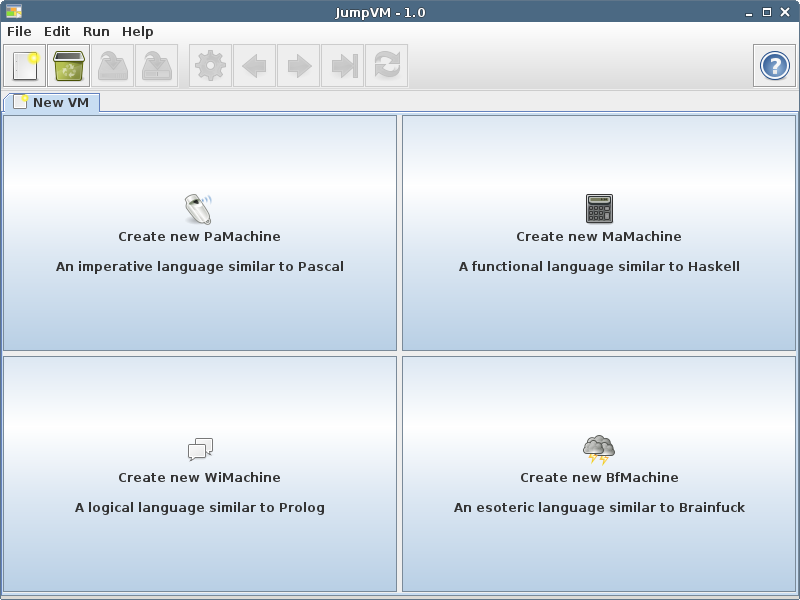
\includegraphics[width=\textwidth]{screenshot_start.png}
    \caption{JumpVM nach dem Start der Software.}
    \label{img_jumpvm_start}
\end{figure}

Der Hilfe-Button auf der rechten Seite öffnet das in Abbildung~\ref{img_jumpvm_help}
zu sehende Fenster mit der Bedienungsanleitung. In dieser
Anleitung findet sich eine generelle Erklärung zum Zweck der Software, eine
Schnellstart-Gebrauchsansweisung, detaillierte Erklärungen zur Funktionsweise
der Menüs und Elemente der Werkzeugleiste, dem visuellen Aufbau der einzelnen
Virtuellen Maschinen und Anmerkungen zu deren jeweiligen Leistungsgrenzen.

\begin{figure}[htb]
    \centering
    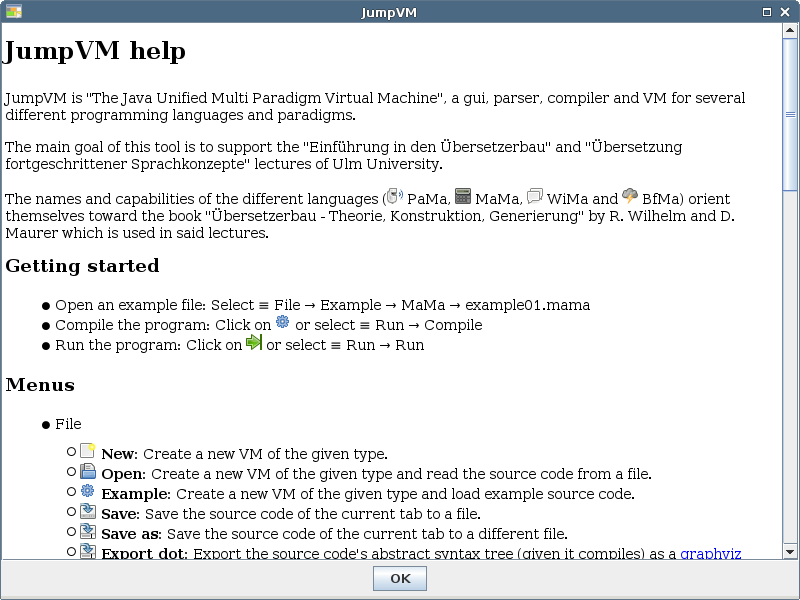
\includegraphics[width=\textwidth]{screenshot_help.png}
    \caption{Auszug aus der Bedienungsanleitung.}
    \label{img_jumpvm_help}
\end{figure}

Öffnet man eine neue Virtuelle Maschine und gibt Quellcode ein, oder verwendet
ein Beispielprogramm aus dem Menü \enquote{File $\rightarrow$ Example}, so kann
man es mit einem Klick auf das Zahnradsymbol \icon{applications-system} oder
den Menüpunkt \enquote{Compile} im Menü \enquote{Run} in Instruktionen der
aktuellen Virtuellen Maschine übersetzen lassen. Durch einen Klick auf das
Symbol \enquote{Pfeil rechts} \icon{go-next} kann das Programm nun
schrittweise, durch einen Klick auf das Symbol \enquote{Pfeil rechts bis Ende}
\icon{go-last} kontinuierlich ausgeführt werden. Das Symbol \enquote{Pfeil
links} \icon{go-previous} macht einen Ausführungsschritt rückgängig, das Symbol
\enquote{Pfeile im Kreis} \icon{view-refresh} setzt die Ausführung zum
Startzustand zurück. Die vier linken Symbole \icon{document-new},
\icon{user-trash}, \icon{document-save} und \icon{document-save-as} dienen zum
Öffnen einer neuen Virtuellen Maschine, dem Schließen der aktuellen Virtuellen
Maschine, dem Speichern des Quellcodes und dem Speichern des Quellcodes unter
einem anderen Namen.

\begin{figure}[htb]
    \centering
    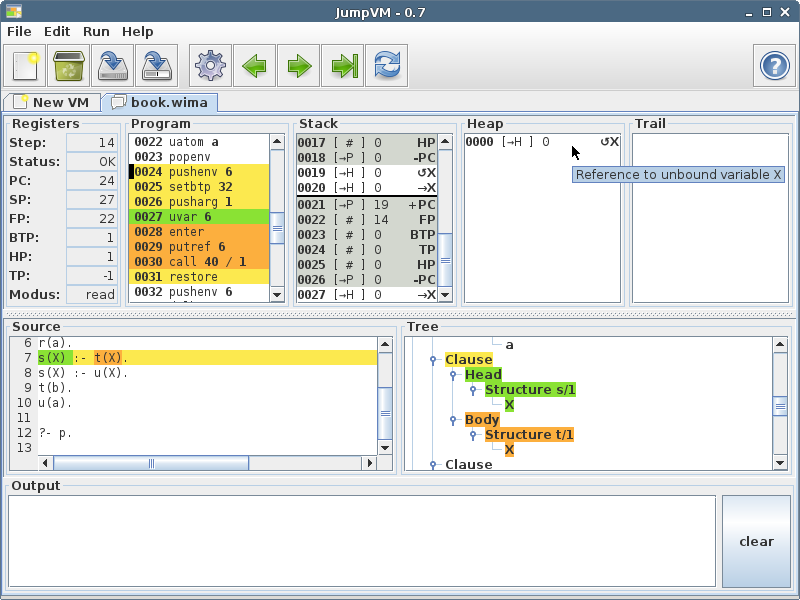
\includegraphics[width=\textwidth]{screenshot.png}
    \caption{Die JumpVM führt ein Programm aus.}
    \label{img_jumpvm_run}
\end{figure}

Abbildung~\ref{img_jumpvm_run} zeigt ein Beispielprogramm während der
Ausführung. Das Feld \enquote{Output} zeigt eventuelle Ausgaben des Programms
an. Diese lassen sich mit dem Knopf \enquote{clear} löschen. Darüber befindet
sich das Feld \enquote{Source}, in dem der Quellcode eingegeben
werden kann. Rechts davon wird im Feld \enquote{Tree} der zugehörige Syntax
Tree des aktuellen compilierten Programms angezeigt.

Im oberen Drittel des Fensters findet sich das Feld \enquote{Registers}, das
die aktuellen Werte der Register der Virtuellen Maschine anzeigt. Daneben
stellt das Feld \enquote{Program} den Programmspeicher, also die erzeugten
Instruktionen für das gegebene Programm dar. Die Felder \enquote{Stack},
\enquote{Heap} und \enquote{Trail} bieten Einblick in die verschiedenen
Arbeitsspeicher der Virtuellen Maschine.

Die farbliche Markierung einiger Elemente in Gelb, Orange und Grün in den
Feldern \enquote{Program}, \enquote{Source} und \enquote{Tree} stellen
semantische Zusammenhänge zwischen dem Quellcode, der Baumdarstellung und den
Maschineninstruktionen dar. Hier wurde beispielsweise auf die Instruktion
\enquote{pushenv 6} im Programmspeicher oder \enquote{Clause} im Syntax Tree
geklickt, wodurch verdeutlicht wird welche Teile Sourcecode welche Teile Syntax
Tree erzeugt und letztendlich welche Instruktionen im Programmcode erzeugt
haben.

Die graue Hinterlegung einiger Einträge im \enquote{Stack}-Speicher markiert
organisatorische Zellen eines Kellerrahmens, dessen Beginn durch einen
schwarzen Strich gekennzeichnet ist. Außerdem ist sichtbar, dass alle
gespeicherten Werte in allen Speichern typisiert und annotiert sind: Etwa
markiert \enquote{$\rightarrow$ P} in Zelle 18 im Stack einen Zeiger auf den
Programmspeicher und \enquote{-PC} für \enquote{Program Counter}
die negative Fortsetzungsadresse des Rahmens. Andere verwendete Symbole sind
zum Beispiel ein durchbrochener Pfeil für einen ungültigen Zeiger und eine Raute für
numerische Werte. Fährt man mit dem Mauscursor über eine Speicherzelle, so wird
die Symbolik der Annotation textuell erklärt.


%%
%% 7. Fazit
%%
\section{Fazit}
Im Wintersemester 2014 wurden im Linux-Rechnerpool der SGI das Betriebssystem
auf Fedora Linux 21, Kernel 3.17.4-302 umgestellt. Die in Kapitel 3 erwähnten
Probleme in der Wartbarkeit kamen zum Tragen und durch die veränderte
Ausführungsumgebung und fehlenden Bibliotheken waren die Programme
pmach, mama und wim nicht mehr ausführbar.

Da die Entwicklung der Software JumpVM zu diesem Zeitpunkt nahezu
fertiggestellt war, konnte der Übungsbetrieb allerdings ohne Unterbrechung
fortgeführt werden. Durch die verwendete Programmiersprache Java und der
gewählten Lizenzierung ist nicht zu erwarten, dass JumpVM in der Zukunft
vergleichbare Probleme haben wird.

Wie in Kapitel 5 dargelegt, wurden die Schwerpunkte aus Kapitel 4 konsequent
umgesetzt und die gesetzten Designziele erreicht und die bisherige
Implementierung der Programme in ihrem Funktionsumfang, ihrer
Benutzerfreundlichkeit und ihrer Fehlertoleranz übertroffen.

Einige Ideen konnten nicht umgesetzt werden, darunter die Entwicklung eines
möglicherweise generischen Backends zur Erzeugung von x86-Assembler bzw.\ der
direkten Erzeugung einer nativen, ausführbaren Datei. Ebenso wurde eine
Visualisierung der Stack- und Heap-Speicher verworfen, da bei vielen Zeigern im
Speicher die Darstellung sehr unübersichtlich würde und die Auswahl konkret
interessanter Zeiger nicht trivial ist.

Eine in der Zukunft mögliche Nachfolgearbeit könnte sich mit der Erweiterung
der JumpVM-Compiler um Optimierungsschritte wie Dead code elimination, Constant
folding oder Loop unrolling beschäftigen.


%%
%% Literatur
%%
\clearpage{}
\printbibliography{}

\end{document}
